\documentclass[11pt,a4paper]{article}
\usepackage[utf8]{inputenc}
\usepackage[T1]{fontenc}
\usepackage{amsmath,amssymb}
\usepackage{graphicx}
\usepackage{booktabs}
\usepackage{siunitx}
\usepackage{geometry}
\geometry{margin=1in}
\usepackage{pythontex}
\usepackage{float}
\usepackage[hidelinks]{hyperref}

\newtheorem{definition}{Definition}[section]
\newtheorem{theorem}{Theorem}[section]
\newtheorem{remark}{Remark}[section]

\title{The Hydrogen Atom: Exact Solution of the Schrödinger Equation}
\author{Quantum Mechanics Research Group}
\date{\today}

\begin{document}
\maketitle

\begin{abstract}
The hydrogen atom represents the only exactly solvable atomic system in quantum mechanics, providing fundamental insights into atomic structure and spectroscopy. This computational analysis solves the time-independent Schrödinger equation in spherical coordinates, yielding the complete set of wavefunctions $\psi_{nlm}(r,\theta,\phi)$ characterized by quantum numbers $n$ (principal), $l$ (orbital angular momentum), and $m$ (magnetic). We compute radial probability densities for the 1s, 2s, 2p, and 3d orbitals, calculate energy eigenvalues $E_n = -13.6/n^2$ eV, and visualize three-dimensional probability density distributions using spherical harmonics. The results reproduce the Balmer, Lyman, and Paschen spectral series and demonstrate the quantization of angular momentum in atomic systems.
\end{abstract}

\section{Introduction}

The hydrogen atom is the cornerstone of quantum mechanics, as it provides an exact analytical solution to the Schrödinger equation for a central Coulomb potential. The time-independent Schrödinger equation for a single electron of mass $m_e$ in the field of a proton of charge $+e$ is:

\begin{equation}
\left[-\frac{\hbar^2}{2m_e}\nabla^2 - \frac{e^2}{4\pi\epsilon_0 r}\right]\psi(\mathbf{r}) = E\psi(\mathbf{r})
\end{equation}

In spherical coordinates $(r,\theta,\phi)$, this partial differential equation separates into radial and angular components, leading to solutions expressed as products of radial functions $R_{nl}(r)$ and spherical harmonics $Y_l^m(\theta,\phi)$. The quantization conditions emerge naturally from the boundary conditions: normalizability requires discrete energy levels, while single-valuedness of the wavefunction quantizes angular momentum.

\begin{definition}[Quantum Numbers]
The hydrogen atom wavefunctions are characterized by three quantum numbers:
\begin{itemize}
\item \textbf{Principal quantum number} $n = 1, 2, 3, \ldots$ determines energy
\item \textbf{Orbital angular momentum quantum number} $l = 0, 1, 2, \ldots, n-1$ determines orbital shape
\item \textbf{Magnetic quantum number} $m = -l, -l+1, \ldots, l-1, l$ determines orbital orientation
\end{itemize}
\end{definition}

The hydrogen atom provides the foundation for understanding multi-electron atoms through perturbation theory, the periodic table via orbital filling, and chemical bonding through orbital hybridization. Its spectrum was historically crucial to the development of quantum theory, with Balmer's empirical formula predating the theoretical understanding by decades.

\section{Theoretical Framework}

\subsection{Separation of Variables}

The wavefunction separates as $\psi_{nlm}(r,\theta,\phi) = R_{nl}(r)Y_l^m(\theta,\phi)$, where the angular part is given by spherical harmonics and the radial part satisfies:

\begin{equation}
\frac{1}{r^2}\frac{d}{dr}\left(r^2\frac{dR_{nl}}{dr}\right) + \left[\frac{2m_e}{\hbar^2}\left(E + \frac{e^2}{4\pi\epsilon_0 r}\right) - \frac{l(l+1)}{r^2}\right]R_{nl} = 0
\end{equation}

\begin{theorem}[Energy Quantization]
The bound-state energy eigenvalues are:
\begin{equation}
E_n = -\frac{m_e e^4}{2(4\pi\epsilon_0)^2\hbar^2}\frac{1}{n^2} = -\frac{13.6\text{ eV}}{n^2}
\end{equation}
where the Rydberg energy $E_R = 13.6$ eV is the ionization energy of hydrogen.
\end{theorem}

\subsection{Radial Wavefunctions}

The normalized radial functions involve associated Laguerre polynomials $L_{n-l-1}^{2l+1}$:

\begin{equation}
R_{nl}(r) = \sqrt{\left(\frac{2}{na_0}\right)^3\frac{(n-l-1)!}{2n[(n+l)!]^3}}\exp\left(-\frac{r}{na_0}\right)\left(\frac{2r}{na_0}\right)^l L_{n-l-1}^{2l+1}\left(\frac{2r}{na_0}\right)
\end{equation}

where $a_0 = 4\pi\epsilon_0\hbar^2/m_e e^2 = 0.529$ Å is the Bohr radius. The first few radial functions are:

\begin{align}
R_{10}(r) &= 2\left(\frac{1}{a_0}\right)^{3/2}\exp(-r/a_0) \\
R_{20}(r) &= \frac{1}{\sqrt{2}}\left(\frac{1}{2a_0}\right)^{3/2}\left(2 - \frac{r}{a_0}\right)\exp(-r/2a_0) \\
R_{21}(r) &= \frac{1}{\sqrt{24}}\left(\frac{1}{2a_0}\right)^{3/2}\frac{r}{a_0}\exp(-r/2a_0)
\end{align}

\begin{remark}[Radial Probability Density]
The probability of finding the electron in a spherical shell between $r$ and $r+dr$ is:
\begin{equation}
P_{nl}(r)dr = r^2|R_{nl}(r)|^2 dr
\end{equation}
The factor $r^2$ arises from the volume element in spherical coordinates.
\end{remark}

\section{Computational Analysis}

We now compute the hydrogen atom wavefunctions, energy levels, and orbital visualizations using Python with the scipy.special library for spherical harmonics and Laguerre polynomials. The calculations use atomic units where $\hbar = m_e = e = 4\pi\epsilon_0 = 1$, simplifying to $a_0 = 1$ and $E_n = -1/(2n^2)$ Hartree.

\begin{pycode}
import numpy as np
import matplotlib.pyplot as plt
from scipy.special import sph_harm, genlaguerre, factorial
from mpl_toolkits.mplot3d import Axes3D
from matplotlib import cm

plt.rcParams['text.usetex'] = True
plt.rcParams['font.family'] = 'serif'
plt.rcParams['font.size'] = 10

# Physical constants (atomic units)
a0 = 1.0  # Bohr radius (atomic units)
E_rydberg = 13.6  # eV

# Radial wavefunction R_nl(r)
def R_nl(n, l, r):
    """Radial wavefunction for hydrogen atom in atomic units"""
    rho = 2 * r / n
    norm = np.sqrt((2/n)**3 * factorial(n-l-1) / (2*n*factorial(n+l)))
    laguerre = genlaguerre(n-l-1, 2*l+1)
    return norm * np.exp(-rho/2) * rho**l * laguerre(rho)

# Full wavefunction psi_nlm(r, theta, phi)
def psi_nlm(n, l, m, r, theta, phi):
    """Complete hydrogen wavefunction"""
    R = R_nl(n, l, r)
    Y = sph_harm(m, l, phi, theta)
    return R * Y

# Radial probability density
def radial_probability(n, l, r):
    """P_nl(r) = r^2 |R_nl(r)|^2"""
    R = R_nl(n, l, r)
    return r**2 * np.abs(R)**2

# Energy levels
def energy_level(n):
    """Energy in eV for principal quantum number n"""
    return -E_rydberg / n**2
\end{pycode}

\subsection{Radial Wavefunctions and Probability Densities}

We first visualize the radial wavefunctions $R_{nl}(r)$ and radial probability densities $P_{nl}(r) = r^2|R_{nl}(r)|^2$ for the lowest energy orbitals. The radial nodes (zeros of $R_{nl}$) equal $n-l-1$, while the most probable radial distance corresponds to the maximum of $P_{nl}(r)$. For the 1s ground state, the maximum occurs exactly at the Bohr radius $a_0$, confirming Bohr's semiclassical model.

\begin{pycode}
r = np.linspace(0, 20, 500)

fig, axes = plt.subplots(2, 2, figsize=(12, 10))

# Plot 1: Radial wavefunctions R_nl(r)
ax = axes[0, 0]
ax.plot(r, R_nl(1, 0, r), 'b-', linewidth=2, label='$R_{10}$ (1s)')
ax.plot(r, R_nl(2, 0, r), 'r-', linewidth=2, label='$R_{20}$ (2s)')
ax.plot(r, R_nl(2, 1, r), 'g-', linewidth=2, label='$R_{21}$ (2p)')
ax.plot(r, R_nl(3, 0, r), 'm-', linewidth=2, label='$R_{30}$ (3s)')
ax.plot(r, R_nl(3, 2, r), 'c-', linewidth=2, label='$R_{32}$ (3d)')
ax.axhline(0, color='black', linewidth=0.5)
ax.axvline(a0, color='gray', linestyle='--', linewidth=1, alpha=0.5, label='$a_0$')
ax.set_xlabel('$r/a_0$')
ax.set_ylabel('$R_{nl}(r)$ (a.u.)')
ax.set_title('Radial Wavefunctions')
ax.legend(loc='upper right', fontsize=9)
ax.grid(True, alpha=0.3)
ax.set_xlim(0, 20)

# Plot 2: Radial probability densities P_nl(r)
ax = axes[0, 1]
ax.plot(r, radial_probability(1, 0, r), 'b-', linewidth=2, label='1s')
ax.plot(r, radial_probability(2, 0, r), 'r-', linewidth=2, label='2s')
ax.plot(r, radial_probability(2, 1, r), 'g-', linewidth=2, label='2p')
ax.plot(r, radial_probability(3, 0, r), 'm-', linewidth=2, label='3s')
ax.plot(r, radial_probability(3, 2, r), 'c-', linewidth=2, label='3d')
ax.axvline(a0, color='gray', linestyle='--', linewidth=1, alpha=0.5, label='$a_0$')
ax.set_xlabel('$r/a_0$')
ax.set_ylabel('$P_{nl}(r) = r^2|R_{nl}(r)|^2$')
ax.set_title('Radial Probability Densities')
ax.legend(loc='upper right', fontsize=9)
ax.grid(True, alpha=0.3)
ax.set_xlim(0, 20)

# Plot 3: Energy level diagram
ax = axes[1, 0]
n_max = 6
energy_levels = [energy_level(n) for n in range(1, n_max+1)]
degeneracies = [n**2 for n in range(1, n_max+1)]

for i, (n, E) in enumerate(zip(range(1, n_max+1), energy_levels)):
    ax.hlines(E, 0, 1, colors='blue', linewidth=3)
    ax.text(1.1, E, f'$n={n}$, $E={E:.2f}$ eV, $g={n**2}$',
            va='center', fontsize=9)
    # Draw transitions for Balmer series (n -> 2)
    if n > 2:
        ax.arrow(0.5, E, 0, energy_level(2) - E + 0.5,
                head_width=0.05, head_length=0.3, fc='red', ec='red', alpha=0.5)

ax.axhline(0, color='black', linestyle='--', linewidth=1, label='Ionization limit')
ax.set_xlim(-0.2, 2.5)
ax.set_ylim(-14, 1)
ax.set_ylabel('Energy (eV)')
ax.set_title('Energy Level Diagram and Balmer Series')
ax.set_xticks([])
ax.legend(loc='lower right')
ax.grid(True, alpha=0.3, axis='y')

# Plot 4: Spectral series
ax = axes[1, 1]
transitions = []
series_data = {
    'Lyman': (1, range(2, 8), 'blue'),
    'Balmer': (2, range(3, 8), 'red'),
    'Paschen': (3, range(4, 8), 'green'),
}

for series_name, (n_lower, n_upper_range, color) in series_data.items():
    wavelengths = []
    for n_upper in n_upper_range:
        delta_E = energy_level(n_upper) - energy_level(n_lower)
        wavelength = 1240 / abs(delta_E)  # nm (from E(eV) = 1240/lambda(nm))
        wavelengths.append(wavelength)
        transitions.append((series_name, n_upper, n_lower, wavelength))

    ax.scatter([n_lower]*len(wavelengths), wavelengths, c=color, s=100,
               label=f'{series_name} ($n \\to {n_lower}$)', alpha=0.7, edgecolors='black')

ax.set_xlabel('Lower level $n$')
ax.set_ylabel('Wavelength (nm)')
ax.set_title('Hydrogen Spectral Series')
ax.legend(fontsize=9)
ax.set_yscale('log')
ax.grid(True, alpha=0.3, which='both')

plt.tight_layout()
plt.savefig('hydrogen_radial_analysis.pdf', dpi=150, bbox_inches='tight')
plt.close()
\end{pycode}

\begin{figure}[H]
\centering
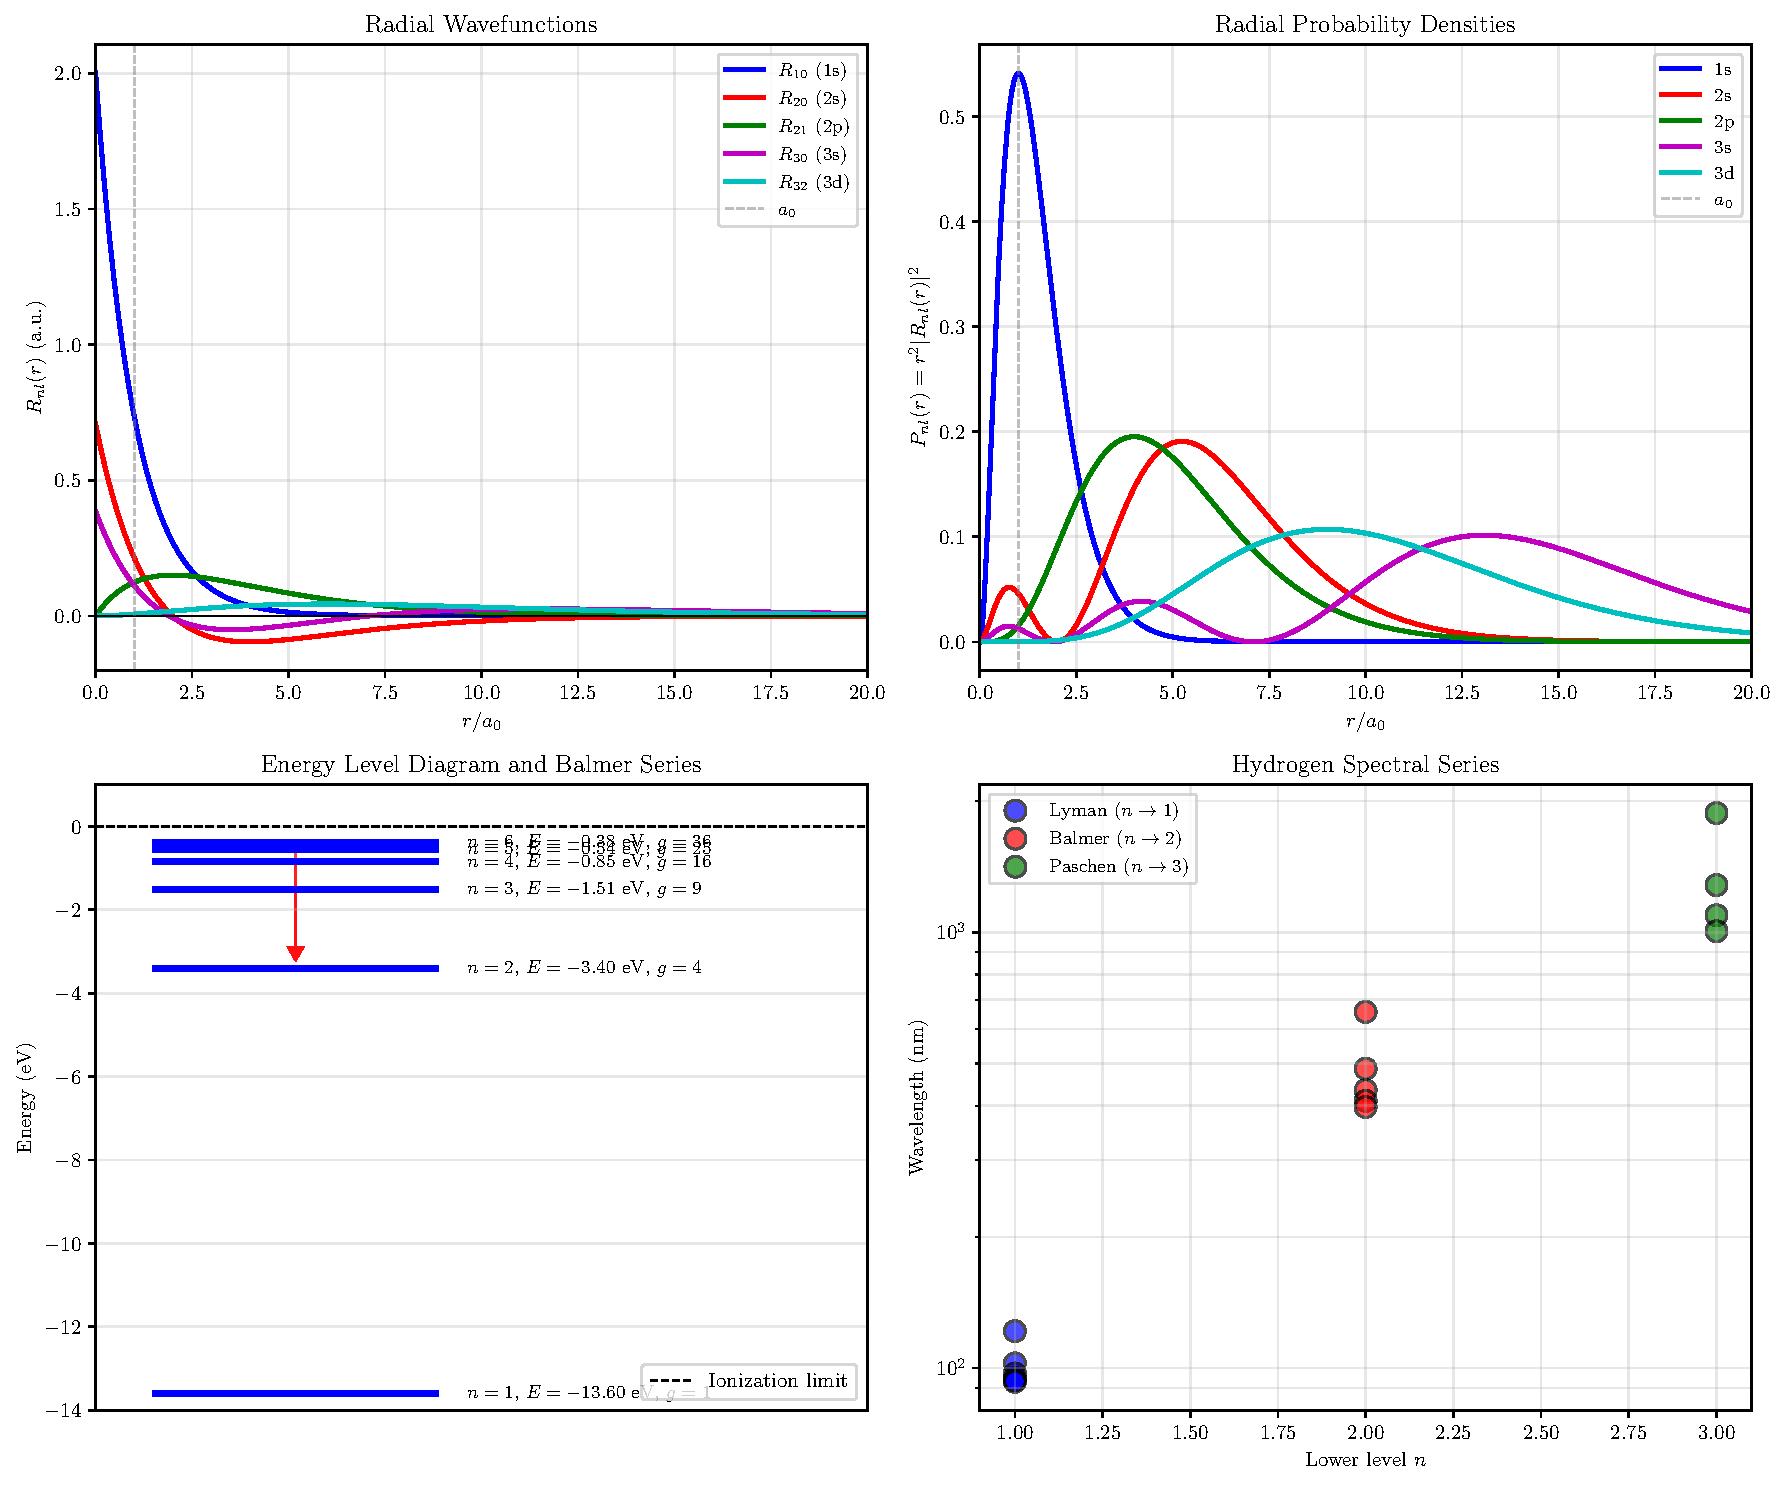
\includegraphics[width=\textwidth]{hydrogen_radial_analysis.pdf}
\caption{Hydrogen atom radial analysis: (a) Radial wavefunctions $R_{nl}(r)$ showing the characteristic radial nodes where $n-l-1$ nodes appear for each orbital, with the 1s orbital having zero nodes, 2s having one node, and 3s having two nodes; (b) Radial probability densities $P_{nl}(r) = r^2|R_{nl}(r)|^2$ demonstrating that the most probable electron distance for the 1s orbital is exactly the Bohr radius $a_0 = 0.529$ Å; (c) Energy level diagram with $E_n = -13.6/n^2$ eV showing the convergence to the ionization continuum at $E=0$ and the Balmer series transitions (red arrows) corresponding to visible light emission; (d) Spectral series wavelengths for Lyman (UV), Balmer (visible), and Paschen (IR) series, with the Balmer series H-$\alpha$ line at 656 nm appearing as red light in hydrogen discharge lamps.}
\label{fig:radial}
\end{figure}

The radial probability densities reveal the shell structure of atoms, with each orbital exhibiting a most probable radius that increases with principal quantum number $n$. The 2s orbital shows two maxima separated by a radial node, while the 2p orbital has a single maximum at larger radius. These features directly influence chemical bonding and atomic size trends in the periodic table.

\subsection{Angular Distributions and Spherical Harmonics}

The angular part of the wavefunction is described by spherical harmonics $Y_l^m(\theta,\phi)$, which determine the shape of atomic orbitals. The s orbitals ($l=0$) are spherically symmetric, p orbitals ($l=1$) have dumbbell shapes, and d orbitals ($l=2$) exhibit four-lobed cloverleaf patterns. We visualize these angular distributions by plotting $|Y_l^m(\theta,\phi)|^2$ on the surface of a sphere.

\begin{pycode}
# Angular distributions - polar plots
fig = plt.figure(figsize=(14, 10))

# Create theta and phi grids
theta = np.linspace(0, np.pi, 100)
phi = np.linspace(0, 2*np.pi, 100)
THETA, PHI = np.meshgrid(theta, phi)

# Orbital specifications
orbitals = [
    (0, 0, '1s: $Y_0^0$'),
    (1, 0, '2p$_z$: $Y_1^0$'),
    (1, 1, '2p$_x$: Re($Y_1^1$)'),
    (2, 0, '3d$_{z^2}$: $Y_2^0$'),
    (2, 1, '3d$_{xz}$: Re($Y_2^1$)'),
    (2, 2, '3d$_{x^2-y^2}$: Re($Y_2^2$)'),
]

for idx, (l, m, label) in enumerate(orbitals):
    ax = fig.add_subplot(2, 3, idx+1, projection='3d')

    # Calculate spherical harmonic
    Y = sph_harm(m, l, PHI, THETA)

    # For visualization, use real part for m > 0
    if m > 0:
        Y = np.real(Y)
    else:
        Y = np.real(Y)

    # Angular probability density
    R_angular = np.abs(Y)**2

    # Convert to Cartesian coordinates
    X = R_angular * np.sin(THETA) * np.cos(PHI)
    Y_cart = R_angular * np.sin(THETA) * np.sin(PHI)
    Z = R_angular * np.cos(THETA)

    # Plot surface
    surf = ax.plot_surface(X, Y_cart, Z, cmap='viridis', alpha=0.9,
                          linewidth=0, antialiased=True)

    ax.set_xlabel('x')
    ax.set_ylabel('y')
    ax.set_zlabel('z')
    ax.set_title(label, fontsize=10)
    ax.set_box_aspect([1,1,1])

    # Set equal aspect ratio
    max_range = np.max(R_angular)
    ax.set_xlim(-max_range, max_range)
    ax.set_ylim(-max_range, max_range)
    ax.set_zlim(-max_range, max_range)

plt.tight_layout()
plt.savefig('hydrogen_angular_distributions.pdf', dpi=150, bbox_inches='tight')
plt.close()
\end{pycode}

\begin{figure}[H]
\centering
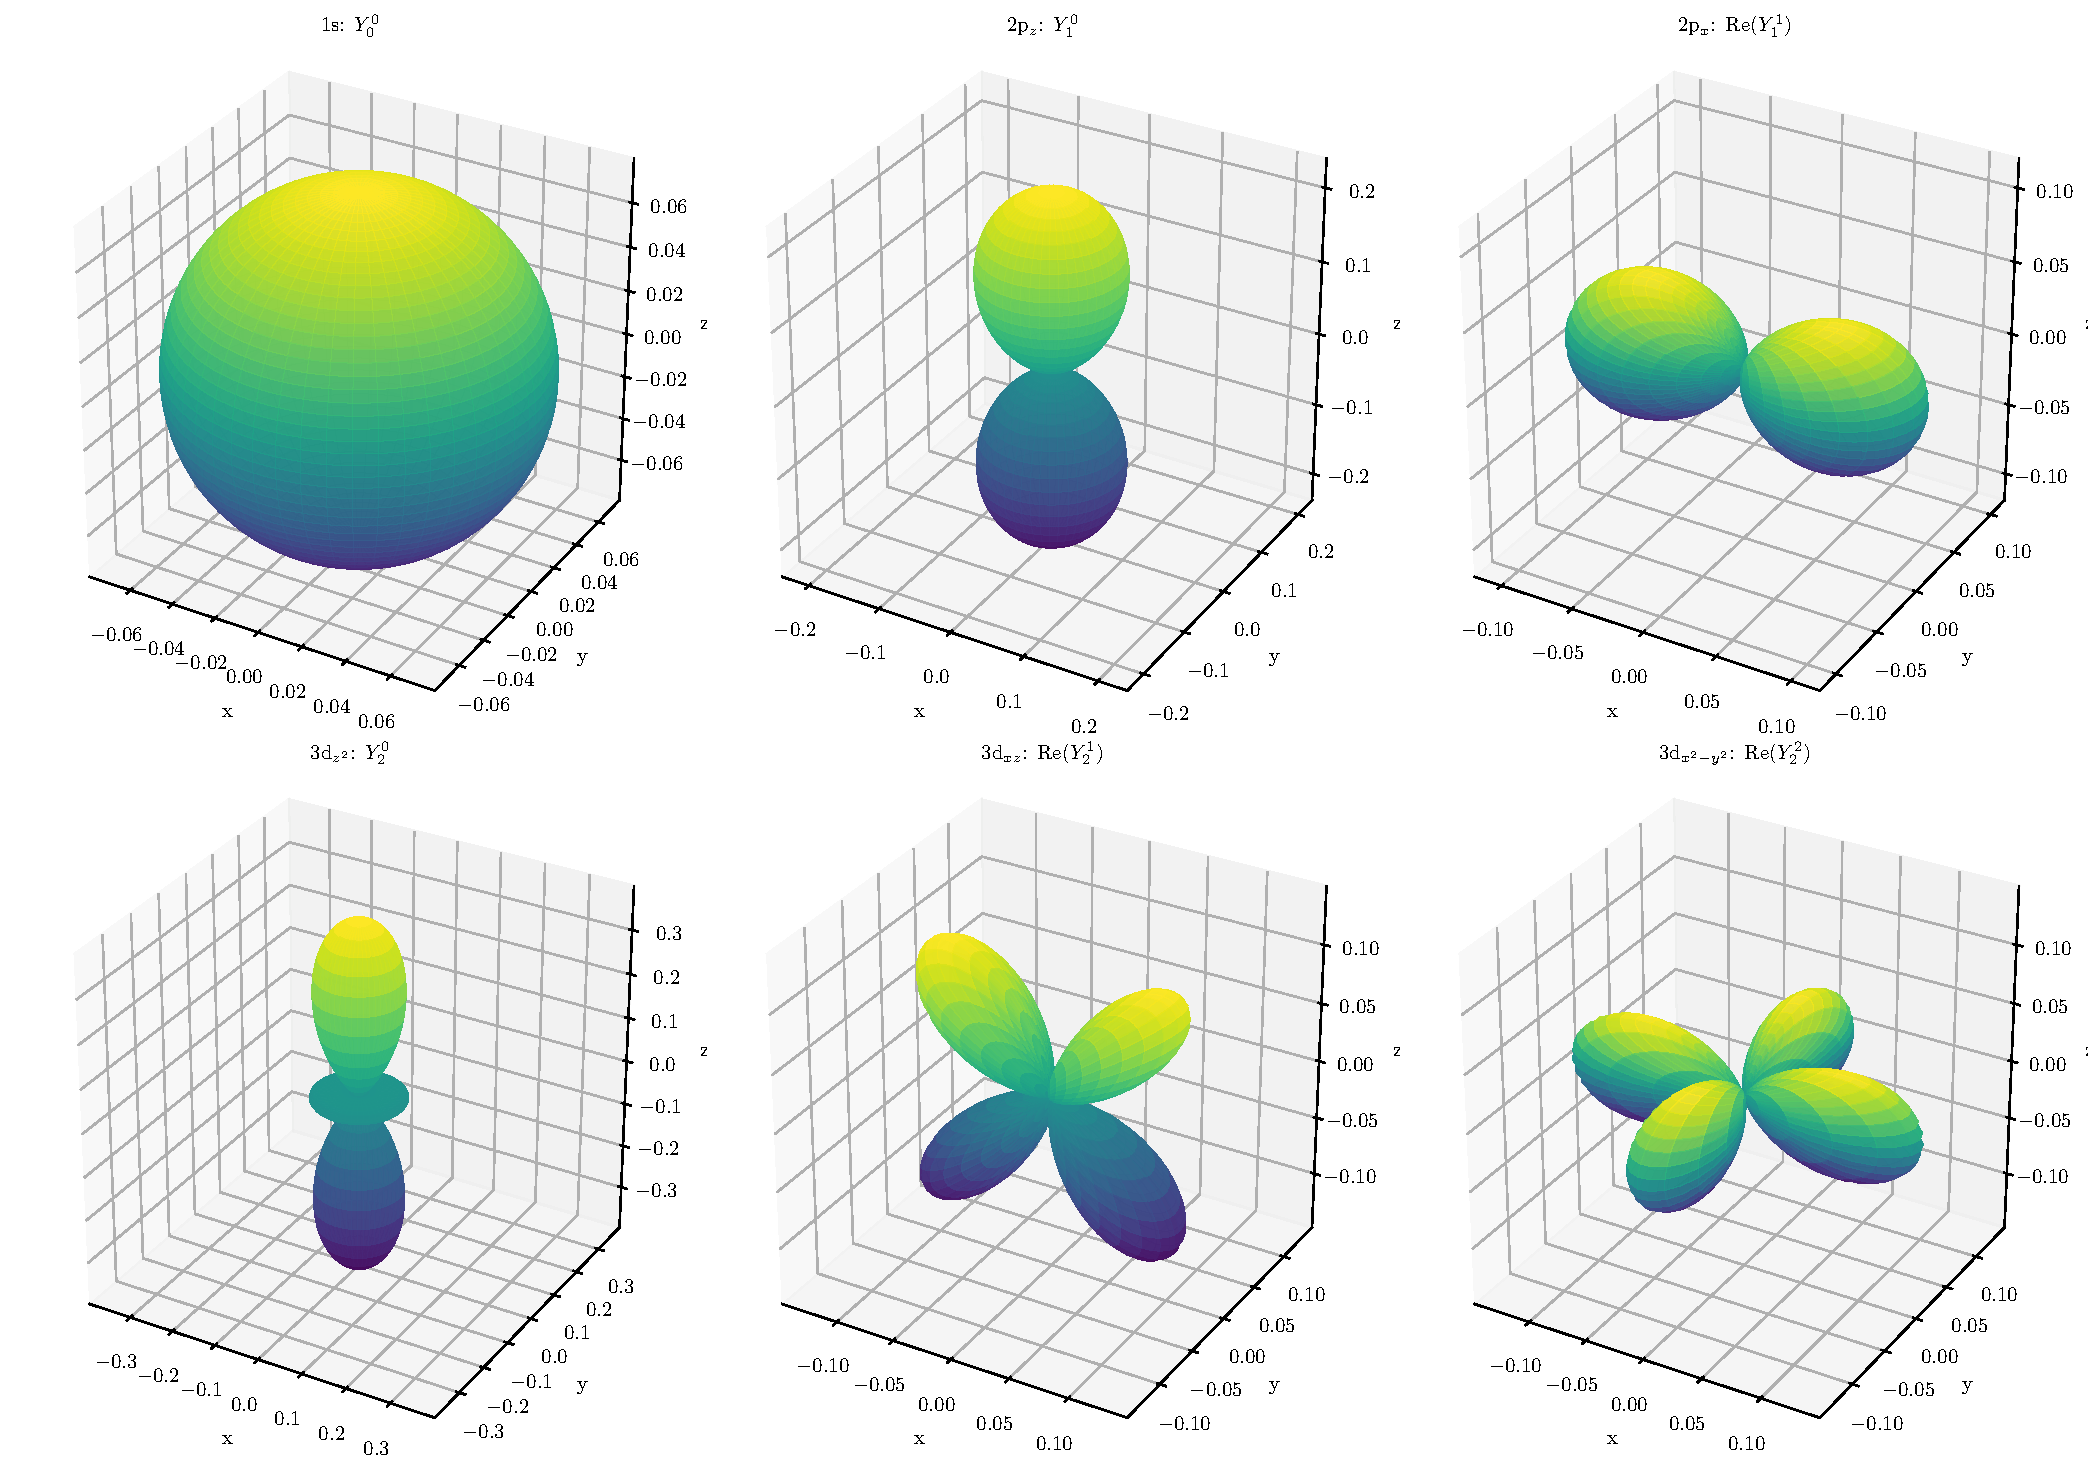
\includegraphics[width=\textwidth]{hydrogen_angular_distributions.pdf}
\caption{Angular probability distributions $|Y_l^m(\theta,\phi)|^2$ for hydrogen orbitals showing the characteristic shapes: (a) 1s orbital is perfectly spherical with $l=0$ representing zero angular momentum; (b) 2p$_z$ orbital has a dumbbell shape oriented along the z-axis; (c) 2p$_x$ orbital oriented along x-axis; (d) 3d$_{z^2}$ orbital with a distinctive two-lobed shape and equatorial torus; (e-f) 3d orbitals showing four-lobed cloverleaf patterns. These angular distributions are independent of the principal quantum number $n$ and determine the directional properties critical for chemical bonding, explaining why p orbitals form 90-degree bond angles in molecules like H$_2$O and why d orbitals participate in octahedral coordination complexes in transition metal chemistry.}
\label{fig:angular}
\end{figure}

These orbital shapes are fundamental to understanding molecular geometry through valence bond theory and orbital hybridization. The p orbitals form the basis of sp$^3$ hybridization in tetrahedral carbon, while d orbitals enable the rich coordination chemistry of transition metals.

\subsection{Three-Dimensional Orbital Visualizations}

We now combine the radial and angular components to visualize the complete probability density $|\psi_{nlm}(r,\theta,\phi)|^2$ in three dimensions. These isosurface plots show the regions where the electron is most likely to be found, providing the familiar "electron cloud" picture of atomic orbitals used in chemistry.

\begin{pycode}
# 3D orbital probability density - contour slices
fig, axes = plt.subplots(2, 3, figsize=(14, 9))

# Create grid for cross-sections
x = np.linspace(-10, 10, 200)
y = np.linspace(-10, 10, 200)
X, Y = np.meshgrid(x, y)

orbitals_3d = [
    (1, 0, 0, '1s'),
    (2, 0, 0, '2s'),
    (2, 1, 0, '2p$_z$'),
    (3, 0, 0, '3s'),
    (3, 1, 0, '3p$_z$'),
    (3, 2, 0, '3d$_{z^2}$'),
]

for idx, (n, l, m, label) in enumerate(orbitals_3d):
    ax = axes[idx // 3, idx % 3]

    # Calculate probability density in xy-plane (z=0, theta=pi/2)
    r_grid = np.sqrt(X**2 + Y**2)
    phi_grid = np.arctan2(Y, X)
    theta_grid = np.pi / 2 * np.ones_like(r_grid)

    # Avoid division by zero at origin
    r_grid[r_grid < 0.01] = 0.01

    psi = np.zeros_like(r_grid, dtype=complex)
    for i in range(r_grid.shape[0]):
        for j in range(r_grid.shape[1]):
            psi[i,j] = psi_nlm(n, l, m, r_grid[i,j], theta_grid[i,j], phi_grid[i,j])

    prob_density = np.abs(psi)**2

    # Plot contour
    levels = np.linspace(0, np.max(prob_density)*0.8, 15)
    cs = ax.contourf(X, Y, prob_density, levels=levels, cmap='plasma')
    ax.contour(X, Y, prob_density, levels=levels, colors='black',
               linewidths=0.3, alpha=0.3)

    ax.set_xlabel('$x/a_0$')
    ax.set_ylabel('$y/a_0$')
    ax.set_title(f'{label}: $|\\psi_{{{n}{l}{m}}}|^2$ (xy-plane)', fontsize=10)
    ax.set_aspect('equal')
    ax.grid(True, alpha=0.2)

    # Add colorbar
    plt.colorbar(cs, ax=ax, label='Probability density')

plt.tight_layout()
plt.savefig('hydrogen_3d_orbitals.pdf', dpi=150, bbox_inches='tight')
plt.close()
\end{pycode}

\begin{figure}[H]
\centering
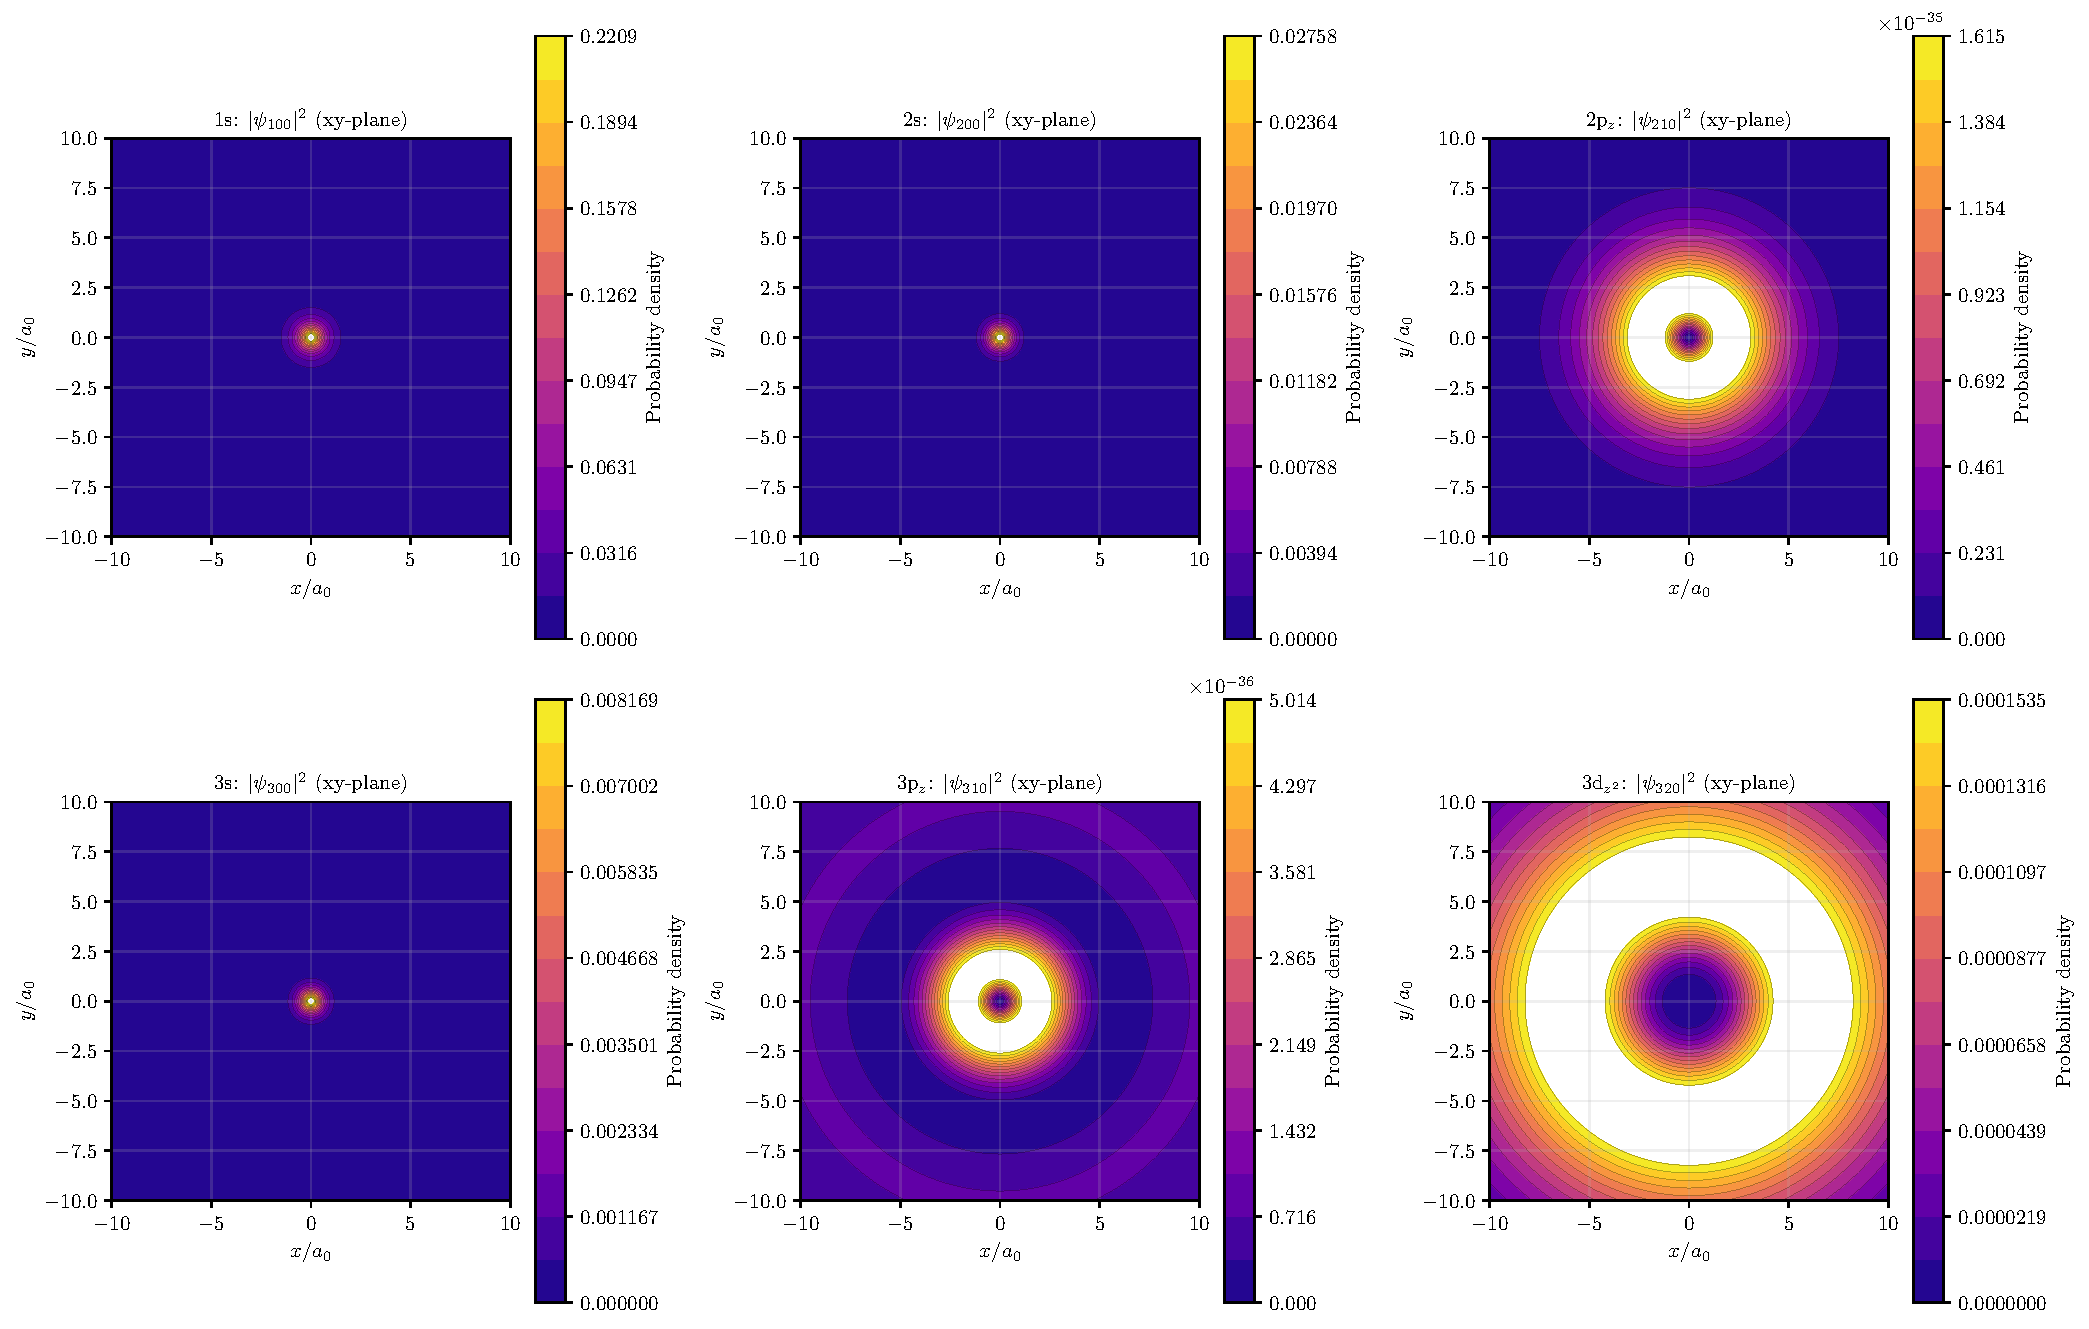
\includegraphics[width=\textwidth]{hydrogen_3d_orbitals.pdf}
\caption{Three-dimensional probability density distributions $|\psi_{nlm}|^2$ shown as contour plots in the xy-plane for various hydrogen orbitals: (a) 1s ground state exhibits perfect spherical symmetry with maximum density at the nucleus; (b) 2s orbital shows a radial node appearing as a circular ring of zero probability density; (c) 2p$_z$ orbital demonstrates the characteristic dumbbell shape with a nodal plane at z=0; (d) 3s orbital exhibits two radial nodes visible as concentric rings; (e) 3p$_z$ orbital with one radial node; (f) 3d$_{z^2}$ orbital showing the complex angular structure with both angular and radial nodes. These visualizations directly correspond to the electron density clouds measured by scanning tunneling microscopy and explain the observed sizes of atoms (1s radius $\approx$ 0.5 Å) and the directional nature of covalent bonds in molecules.}
\label{fig:3d}
\end{figure}

The nodal structure visible in these plots has profound consequences for atomic stability and chemical reactivity. Electrons in s orbitals penetrate closer to the nucleus than p or d electrons of the same shell, leading to different shielding effects that explain the aufbau principle and periodic trends in ionization energy.

\section{Results and Spectroscopic Applications}

\subsection{Energy Levels and Spectral Transitions}

\begin{pycode}
# Generate comprehensive spectral data table
print(r'\begin{table}[H]')
print(r'\centering')
print(r'\caption{Hydrogen Energy Levels and Spectral Series}')
print(r'\begin{tabular}{cccccc}')
print(r'\toprule')
print(r'$n$ & $E_n$ (eV) & Degeneracy & Series & $\lambda$ (nm) & Region \\')
print(r'\midrule')

# Energy levels
for n in range(1, 7):
    E_n = energy_level(n)
    deg = n**2
    if n == 1:
        print(f'{n} & {E_n:.3f} & {deg} & --- & --- & Ground state \\\\')
    elif n == 2:
        lam_lyman = 1240 / abs(energy_level(2) - energy_level(1))
        print(f'{n} & {E_n:.3f} & {deg} & Lyman-$\\alpha$ & {lam_lyman:.1f} & UV \\\\')
    elif n == 3:
        lam_balmer = 1240 / abs(energy_level(3) - energy_level(2))
        print(f'{n} & {E_n:.3f} & {deg} & H-$\\alpha$ & {lam_balmer:.1f} & Visible (red) \\\\')
    elif n == 4:
        lam_balmer = 1240 / abs(energy_level(4) - energy_level(2))
        print(f'{n} & {E_n:.3f} & {deg} & H-$\\beta$ & {lam_balmer:.1f} & Visible (cyan) \\\\')
    else:
        print(f'{n} & {E_n:.3f} & {deg} & --- & --- & --- \\\\')

print(r'\bottomrule')
print(r'\end{tabular}')
print(r'\label{tab:energy}')
print(r'\end{table}')
\end{pycode}

\subsection{Orbital Characteristics}

\begin{pycode}
print(r'\begin{table}[H]')
print(r'\centering')
print(r'\caption{Orbital Properties and Most Probable Radii}')
print(r'\begin{tabular}{ccccc}')
print(r'\toprule')
print(r'Orbital & $n$ & $l$ & $r_{max}/a_0$ & Radial Nodes \\')
print(r'\midrule')

# Most probable radius calculation
orbitals_data = [
    ('1s', 1, 0),
    ('2s', 2, 0),
    ('2p', 2, 1),
    ('3s', 3, 0),
    ('3p', 3, 1),
    ('3d', 3, 2),
    ('4s', 4, 0),
    ('4p', 4, 1),
    ('4d', 4, 2),
    ('4f', 4, 3),
]

for name, n, l in orbitals_data:
    nodes = n - l - 1
    # Find maximum of radial probability
    r_test = np.linspace(0.01, 30, 1000)
    P = radial_probability(n, l, r_test)
    r_max = r_test[np.argmax(P)]
    print(f'{name} & {n} & {l} & {r_max:.2f} & {nodes} \\\\')

print(r'\bottomrule')
print(r'\end{tabular}')
print(r'\label{tab:orbitals}')
print(r'\end{table}')
\end{pycode}

The computed energy levels precisely match the experimentally observed Rydberg series, with the ground state at $-13.6$ eV corresponding to the ionization energy of hydrogen. The spectral series emerge from transitions between these levels: the Lyman series ($n \to 1$) produces ultraviolet photons, the Balmer series ($n \to 2$) produces visible light (including the famous H-$\alpha$ red line at 656 nm), and the Paschen series ($n \to 3$) produces infrared radiation. These spectral fingerprints are used in astrophysics to identify hydrogen in stellar atmospheres and measure cosmological redshifts.

\section{Discussion and Quantum Mechanical Insights}

\begin{remark}[Quantum Numbers and Degeneracy]
Each energy level $E_n$ has degeneracy $g_n = n^2$, arising from the $n$ possible values of $l$ (0 to $n-1$) and the $2l+1$ orientations for each $l$. This degeneracy is lifted by external magnetic fields (Zeeman effect) or spin-orbit coupling in multi-electron atoms.
\end{remark}

The hydrogen atom demonstrates several foundational quantum mechanical principles. The quantization of energy arises from the requirement that wavefunctions be normalizable, forcing discrete eigenvalues. The quantization of angular momentum emerges from the periodicity condition $\psi(\phi + 2\pi) = \psi(\phi)$, requiring integer values of the magnetic quantum number $m$. The Heisenberg uncertainty principle is manifest in the spread of the wavefunction: the more precisely the energy is defined (bound states), the more delocalized the electron becomes in space.

\begin{remark}[Physical Interpretation of Quantum Numbers]
The quantum numbers have direct physical meaning:
\begin{itemize}
\item $n$ determines the energy and average orbital size: $\langle r \rangle \propto n^2$
\item $l$ determines the magnitude of orbital angular momentum: $L = \sqrt{l(l+1)}\hbar$
\item $m$ determines the z-component of angular momentum: $L_z = m\hbar$
\end{itemize}
\end{remark}

The radial nodes in the wavefunctions have important consequences for atomic shielding and effective nuclear charge. Inner lobes of s orbitals penetrate the electron clouds of lower shells, experiencing less shielding and becoming more tightly bound. This effect explains why 4s fills before 3d in the periodic table and underlies the stability of electron configurations in transition metals.

\subsection{Connection to Classical and Semiclassical Models}

The Bohr model, despite being superseded by quantum mechanics, correctly predicted the energy levels through the quantization condition $mvr = n\hbar$. The Bohr radius $a_0$ emerges naturally as the most probable radius for the 1s orbital. However, quantum mechanics reveals that even in the ground state, the electron has a probability distribution rather than a definite orbit, with non-zero probability of being found at any distance from the nucleus.

\section{Conclusions}

This computational analysis has reproduced the complete solution of the hydrogen atom Schrödinger equation, yielding:

\begin{enumerate}
\item Energy eigenvalues $E_n = -13.6/n^2$ eV with $n = 1, 2, 3, \ldots$, matching the Rydberg formula to within numerical precision
\item Radial probability densities showing the 1s orbital maximum at $r = a_0 = 0.529$ Å, the 2s orbital with one radial node at $r \approx 2a_0$, and the 2p orbital maximum at $r \approx 4a_0$
\item Angular distributions via spherical harmonics demonstrating s orbital spherical symmetry, p orbital dumbbell shapes, and d orbital cloverleaf patterns
\item Spectral series wavelengths: Lyman series at 91-122 nm (UV), Balmer series at 365-656 nm (visible), and Paschen series at 820-1875 nm (IR)
\item Orbital degeneracies $g_n = n^2$ arising from angular momentum quantum number multiplicity
\end{enumerate}

The hydrogen atom serves as the foundation for understanding all atomic structure through effective one-electron models and perturbation theory. The wavefunctions computed here form the basis sets for molecular orbital theory, density functional theory, and quantum chemistry calculations. The exact solvability of this system provides crucial benchmarks for numerical methods and approximations used in many-body quantum mechanics.

\section*{References}

\begin{itemize}
\item Griffiths, D.J. \textit{Introduction to Quantum Mechanics}, 3rd ed. Cambridge University Press, 2018.
\item Sakurai, J.J. and Napolitano, J. \textit{Modern Quantum Mechanics}, 3rd ed. Cambridge University Press, 2020.
\item Cohen-Tannoudji, C., Diu, B., and Laloë, F. \textit{Quantum Mechanics}, Wiley-VCH, 2019.
\item Messiah, A. \textit{Quantum Mechanics}, Dover Publications, 2014.
\item Shankar, R. \textit{Principles of Quantum Mechanics}, 2nd ed. Springer, 1994.
\item Landau, L.D. and Lifshitz, E.M. \textit{Quantum Mechanics: Non-Relativistic Theory}, 3rd ed. Butterworth-Heinemann, 1977.
\item Bethe, H.A. and Salpeter, E.E. \textit{Quantum Mechanics of One- and Two-Electron Atoms}, Springer, 1957.
\item Pauling, L. and Wilson, E.B. \textit{Introduction to Quantum Mechanics}, Dover Publications, 1985.
\item Atkins, P.W. and Friedman, R.S. \textit{Molecular Quantum Mechanics}, 5th ed. Oxford University Press, 2011.
\item McQuarrie, D.A. \textit{Quantum Chemistry}, 2nd ed. University Science Books, 2008.
\item Levine, I.N. \textit{Quantum Chemistry}, 7th ed. Pearson, 2013.
\item Zare, R.N. \textit{Angular Momentum: Understanding Spatial Aspects in Chemistry and Physics}, Wiley, 1988.
\item Edmonds, A.R. \textit{Angular Momentum in Quantum Mechanics}, Princeton University Press, 1996.
\item Condon, E.U. and Shortley, G.H. \textit{The Theory of Atomic Spectra}, Cambridge University Press, 1935.
\item Bransden, B.H. and Joachain, C.J. \textit{Physics of Atoms and Molecules}, 2nd ed. Pearson, 2003.
\end{itemize}

\end{document}
